\appendix
\chapter{Anhang}
\section{Anwendungsfallbeschreibung}
\label{anhang:anwendungsfallbeschreibung}
\subsection{Neues Page Object anlegen}
\label{sec:neues_page_object_anlegen}

\begin{tabular}[h]{|p{4cm}|p{11,5cm}|}
\hline 
\rule[-1ex]{0pt}{2.5ex}Kurzbeschreibung: & 
Entwickler legt ein neues Page Object an. \\  
\hline 
\rule[-1ex]{0pt}{2.5ex}Akteure: & 
Entwickler \\ 
\hline 
\rule[-1ex]{0pt}{2.5ex}Motivation: & 
Entwickler benötigt Page Object in den Testfällen. \\ 
\hline 
\rule[-1ex]{0pt}{2.5ex}Vorbedingung: &  \\ 
\hline 
\rule[-1ex]{0pt}{2.5ex}Eingehende Daten: & Name und Paket des Page Object. \\ 
\hline 
\rule[-1ex]{0pt}{2.5ex}Ergebnisse: & Page Object ist ausgewählt. \\ 
\hline 
\rule[-1ex]{0pt}{2.5ex}Nachbedingungen: & Page Object wurde im Modell der Anwendung angelegt.  \\ 
\hline 
\end{tabular} 

\paragraph{Ablauf}

\begin{itemize}[itemsep=0pt]
\item[1.] Entwickler startet den Vorgang zum Anlegen eines neuen Page Object. 
\item[2.] System zeigt Dialog an. 
\item[3.] Entwickler trägt Namen des Page Object im Dialog ein.
\item[4.] Entwickler bestätigt den Dialog.
\item[5.] System prüft Eingaben.
\item[6.] System wählt Page Object aus.
\end{itemize}

\paragraph{Vorgang abgebrochen}
Statt Schritt 4-6:
\begin{itemize}[itemsep=0pt]
\item[4.] Entwickler bricht Vorgang ab. 
\item[5.] System ändert internen Zustand nicht. 
\end{itemize}

\paragraph{Validierung fehlgeschlagen}
Statt Schritt 6:
\begin{itemize}[itemsep=0pt]
\item[6.] System zeigt Fehlermeldung an. 
\item[7.] Entwickler bestätigt Fehlermeldung. 
\end{itemize}
Weiter mit Punkt 3. 

\paragraph{Paketstruktur des Page Object verfeinern}
Statt Schritt 4:
\begin{itemize}[itemsep=0pt]
\item[4.] Entwickler trägt Paket des Page Object ein.
\end{itemize}
Weiter mit Punkt 4. 
 

\subsection{Neues Element hinzufügen}
\label{sec:neues_element_hinzufügen}

\begin{tabular}[h]{|p{4cm}|p{11,5cm}|}
\hline 
\rule[-1ex]{0pt}{2.5ex}Kurzbeschreibung: & 
Entwickler legt ein Element in einem Page Object an. \\  
\hline 
\rule[-1ex]{0pt}{2.5ex}Akteure: & 
Entwickler \\ 
\hline 
\rule[-1ex]{0pt}{2.5ex}Motivation: & 
Entwickler benötigt Element der Seite in den Testfällen. \\ 
\hline 
\rule[-1ex]{0pt}{2.5ex}Vorbedingung: & 
Page Object bereits angelegt.\\ 
\hline 
\rule[-1ex]{0pt}{2.5ex}Eingehende Daten: & Interner Name des Elements, Art des Selektors, Locator, der das Element in der Seite identifiziert \\ 
\hline 
\rule[-1ex]{0pt}{2.5ex}Ergebnisse: & Element wird in den Elementen des Page Object angezeigt. \\ 
\hline 
\rule[-1ex]{0pt}{2.5ex}Nachbedingungen: & Element wurde im Modell der Anwendung angelegt.  \\ 
\hline 
\end{tabular} 

\paragraph{Ablauf}

\begin{itemize}[itemsep=0pt]
\item[1.] Entwickler wählt Page Object aus.
\item[2.] Entwickler wählt Bereich für die Elemente des Page Objects aus. 
\item[3.] System wechselt in den internen Zustand zum Bearbeiten von Elementen.
\item[4.] Entwickler startet den Vorgang zum Anlegen eines neuen Eintrags.
\item[5.] System zeigt Dialog an. 
\item[6.] Entwickler befüllt Dialog.
\item[7.] Entwickler bestätigt den Dialog.
\item[8.] System prüft, ob alle Felder befüllt sind.
\item[9.] System zeigt Element in den Elementen des Page Object an.
\end{itemize}

\paragraph{Vorgang abgebrochen}
Statt Schritt 7-9:
\begin{itemize}[itemsep=0pt]
\item[7.] Entwickler bricht Vorgang ab. 
\item[8.] System ändert internen Zustand nicht. 
\end{itemize}

\paragraph{Validierung fehlgeschlagen}
Statt Schritt 9:
\begin{itemize}
\item[9.] System zeigt Fehlermeldung an. 
\item[10.] Entwickler bestätigt Fehlermeldung. 
\end{itemize}
Weiter mit Punkt 6. 


\subsection{Neue Transition hinzufügen}
\label{sec:neue_transition_hinzufügen}

\begin{tabular}[h]{|p{4cm}|p{11,5cm}|}
\hline 
\rule[-1ex]{0pt}{2.5ex}Kurzbeschreibung: & 
Entwickler legt einen Seitenübergang zu einem anderen Page Object an. \\  
\hline 
\rule[-1ex]{0pt}{2.5ex}Akteure: & 
Entwickler \\ 
\hline 
\rule[-1ex]{0pt}{2.5ex}Motivation: & 
Entwickler benötigt einen Übergang zu einer anderen Seite in den Testfällen. \\ 
\hline 
\rule[-1ex]{0pt}{2.5ex}Vorbedingung: & 
Page Object bereits angelegt. Page Object, das Ziel des Seitenübergangs ist, wurde bereits angelget.\\ 
\hline 
\rule[-1ex]{0pt}{2.5ex}Eingehende Daten: & Interner Name des Elements, Art des Selektors, Locator der das Element in der Seite identifiziert, Ziel Page Object. \\ 
\hline 
\rule[-1ex]{0pt}{2.5ex}Ergebnisse: & Transition wird in den Transitionen des Page Object angezeigt. \\ 
\hline 
\rule[-1ex]{0pt}{2.5ex}Nachbedingungen: & Transition wurde im Modell der Anwendung angelegt.  \\ 
\hline 
\end{tabular} 

\paragraph{Ablauf}

\begin{itemize}[itemsep=0pt]
\item[1.] Entwickler wählt Page Object aus.
\item[2.] Entwickler wählt Bereich für die Transitionen des Page Objects aus. 
\item[3.] System wechselt in den internen Zustand zum Bearbeiten von Transitionen.
\item[4.] Entwickler startet den Vorgang zum Anlegen eines neuen Eintrags.
\item[5.] System zeigt Dialog an. 
\item[6.] Entwickler befüllt Dialog.
\item[7.] Entwickler bestätigt den Dialog.
\item[8.] System prüft ob alle Felder befüllt sind.
\item[9.] System zeigt Transition in den Transitionen des Page Object an.
\end{itemize}

\paragraph{Vorgang abgebrochen}
Statt Schritt 7-9:
\begin{itemize}[itemsep=0pt]
\item[7.] Entwickler bricht Vorgang ab. 
\item[8.] System ändert internen Zustand nicht. 
\end{itemize}

\paragraph{Validierung fehlgeschlagen}
Statt Schritt 9:
\begin{itemize}
\item[9.] System zeigt Fehlermeldung an. 
\item[10.] Entwickler bestätigt Fehlermeldung. 
\end{itemize}
Weiter mit Punkt 6. 


\subsection{Element aus HTML übernehmen}
\label{sec:element_from_html}

\begin{tabular}[h]{|p{4cm}|p{11,5cm}|}
\hline 
\rule[-1ex]{0pt}{2.5ex}Kurzbeschreibung: & 
Entwickler legt teilautomatisiert ein neues Element im Page Object an. \\  
\hline 
\rule[-1ex]{0pt}{2.5ex}Akteure: & 
Entwickler \\ 
\hline 
\rule[-1ex]{0pt}{2.5ex}Motivation: & 
Entwickler benötigt Element der Seite in den Testfällen. \\ 
\hline 
\rule[-1ex]{0pt}{2.5ex}Vorbedingung: & 
Page Object bereits angelegt. \\ 
\hline 
\rule[-1ex]{0pt}{2.5ex}Eingehende Daten: & Art des Locators, nach dem die Seite durchsucht werden soll. \\ 
\hline 
\rule[-1ex]{0pt}{2.5ex}Ergebnisse: & Element wird in den Elementen des Page Object angezeigt. \\ 
\hline 
\rule[-1ex]{0pt}{2.5ex}Nachbedingungen: & Element wurde im Modell der Anwendung angelegt.  \\ 
\hline 
\end{tabular} 

\paragraph{Ablauf}

\begin{itemize}[itemsep=0pt]
\item[1.] Entwickler wählt Page Object aus.
\item[2.] Entwickler startet aus der Anwendung heraus den Webbrowser mit der zum ausgewählten Page Object korrespondierenden Seite. 
\item[3.] Entwickler wählt Art des Locators, für den die Seite durchsucht werden soll, aus.
\item[4.] Entwickler wählt Aktion zum Analysieren der ausgewählten Webseite aus.
\item[5.] System zeigt die für den ausgewählten Locator auf der Seite identifizierten Elemente an.
\item[6.] Entwickler wählt gewünschtes Element aus den Treffern aus. 
\item[7.] Entwickler wählt Aktion zum Übernehmen des Elements in das Page Object aus.
\item[8.] System zeigt Element in den Elementen des Page Object an.
\end{itemize}

\paragraph{Testen des Elements}
Statt Schritt 7-8:
\begin{itemize}
\item[7.] Entwickler wählt Aktion zum Testen des ausgewählten Elements aus. 
\item[8.] System zeigt an, ob das Element auf der ausgewählten Webseite erfolgreich erreicht werden konnte. 
\end{itemize}
Weiter mit Punkt 7. 

\subsection{Transition aus HTML übernehmen}
\label{sec:Transition_from_html}

\begin{tabular}[h]{|p{4cm}|p{11,5cm}|}
\hline 
\rule[-1ex]{0pt}{2.5ex}Kurzbeschreibung: & 
Entwickler legt teilautomatisiert einen neuen Seitenübergang an. \\  
\hline 
\rule[-1ex]{0pt}{2.5ex}Akteure: & 
Entwickler \\ 
\hline 
\rule[-1ex]{0pt}{2.5ex}Motivation: & 
Entwickler benötigt einen Übergang zu einer anderen Seite in den Testfällen. \\ 
\hline 
\rule[-1ex]{0pt}{2.5ex}Vorbedingung: & 
Page Object bereits angelegt. Page Object, das Ziel des Seitenübergangs ist, wurde bereits angelget. \\ 
\hline 
\rule[-1ex]{0pt}{2.5ex}Eingehende Daten: & Art des Locators nach dem die Seite durchsucht werden soll, Ziel Page Object. \\ 
\hline 
\rule[-1ex]{0pt}{2.5ex}Ergebnisse: & Transition wird in den Transitionen des Page Object angezeigt. \\ 
\hline 
\rule[-1ex]{0pt}{2.5ex}Nachbedingungen: & Transition wurde im Modell der Anwendung angelegt.  \\ 
\hline 
\end{tabular} 

\paragraph{Ablauf}

\begin{itemize}[itemsep=0pt]
\item[1.] Entwickler wählt passendes Page Object aus.
\item[2.] Entwickler startet aus der Anwendung heraus den Webbrowser mit der zum ausgewählten Page Object korrespondierenden Seite. 
\item[3.] Entwickler wählt Art des Locators, für den die Seite durchsucht werden soll, aus.
\item[4.] Entwickler wählt Aktion zum Analysieren der ausgewählten Webseite aus.
\item[5.] System zeigt die für den ausgewählten Locator auf der Seite identifizierten Elemente an.
\item[6.] Entwickler wählt gewünschtes Element aus den Treffern aus. 
\item[7.] Entwickler wählt Aktion zum Übernehmen des Elements als Transition in das Page Object aus.
\item[8.] System zeigt Dialog mit den Informationen des ausgewählten Elements an.
\item[9.] Entwickler ergänzt die Informationen um das Ziel Page Object der Transition.
\item[10.] Entwickler bestätigt den Dialog.
\item[11.] System prüft, ob alle Felder befüllt sind.
\item[12.] System zeigt Element in den Transitionen des Page Object an.
\end{itemize}

\paragraph{Testen der Transition}
Statt Schritt 7-12:
\begin{itemize}
\item[7.] Entwickler wählt Aktion zum Testen des ausgewählten Elements aus. 
\item[8.] System zeigt an, ob das Element auf der ausgewählten Webseite erfolgreich erreicht werden konnte. 
\end{itemize}
Weiter mit Punkt 7.

\paragraph{Vorgang abgebrochen}
Statt Schritt 10-12:
\begin{itemize}[itemsep=0pt]
\item[10.] Entwickler bricht Vorgang ab. 
\item[11.] System ändert internen Zustand nicht. 
\end{itemize}

\paragraph{Validierung fehlgeschlagen}
Statt Schritt 12:
\begin{itemize}
\item[12.] System zeigt Fehlermeldung an. 
\item[13.] Entwickler bestätigt Fehlermeldung. 
\end{itemize}
Weiter mit Punkt 6. 


\subsection{Vorhandenen Eintrag editieren}
\label{sec:edit_entry}

\begin{tabular}[h]{|p{4cm}|p{11,5cm}|}
\hline 
\rule[-1ex]{0pt}{2.5ex}Kurzbeschreibung: & 
Entwickler editiert bereits vorhandenen Eintrag. \\  
\hline 
\rule[-1ex]{0pt}{2.5ex}Akteure: & 
Entwickler \\ 
\hline 
\rule[-1ex]{0pt}{2.5ex}Motivation: & 
Entwickler möchte einen bereits vorhandenen Eintrag überarbeiten. \\ 
\hline 
\rule[-1ex]{0pt}{2.5ex}Vorbedingung: & 
Eintrag bereits vorhanden. \\ 
\hline 
\rule[-1ex]{0pt}{2.5ex}Eingehende Daten: & Geänderte Werte. \\ 
\hline 
\rule[-1ex]{0pt}{2.5ex}Ergebnisse: & Eintrag wird in aktualisierter Form angezeigt. \\ 
\hline 
\rule[-1ex]{0pt}{2.5ex}Nachbedingungen: & Eintrag wurde im Modell der Anwendung aktualisiert.  \\ 
\hline 
\end{tabular} 

\paragraph{Ablauf}

\begin{itemize}[itemsep=0pt]
\item[1.] Entwickler wählt den zu editierenden Eintrag aus.
\item[2.] Entwickler löst die Aktion zum Editieren der aktuellen Auswahl aus. 
\item[3.] System zeigt Dialog mit den aktuellen Werten des Eintrags an.
\item[4.] Entwickler nimmt die gewünschten Änderungen vor.
\item[5.] Entwickler bestätigt den Dialog.
\item[6.] System prüft die Felder des Dialogs.
\item[7.] System zeigt den Eintrag in aktualisierter Form an.
\end{itemize}

\paragraph{Vorgang abgebrochen}
Statt Schritt 5-7:
\begin{itemize}[itemsep=0pt]
\item[5.] Entwickler bricht Vorgang ab. 
\item[6.] System ändert internen Zustand nicht. 
\end{itemize}

\paragraph{Validierung fehlgeschlagen}
Statt Schritt 7:
\begin{itemize}[itemsep=0pt]
\item[7.] System zeigt Fehlermeldung an. 
\item[8.] Entwickler bestätigt Fehlermeldung. 
\end{itemize}
Weiter mit Punkt 4. 

\subsection{Vorhandenen Eintrag löschen}
\label{sec:delete_entry}

\begin{tabular}[h]{|p{4cm}|p{11,5cm}|}
\hline 
\rule[-1ex]{0pt}{2.5ex}Kurzbeschreibung: & 
Entwickler löscht bereits vorhandenen Eintrag. \\  
\hline 
\rule[-1ex]{0pt}{2.5ex}Akteure: & 
Entwickler \\ 
\hline 
\rule[-1ex]{0pt}{2.5ex}Motivation: & 
Entwickler möchte einen bereits vorhandenen Eintrag löschen. \\ 
\hline 
\rule[-1ex]{0pt}{2.5ex}Vorbedingung: & 
Eintrag bereits vorhanden. \\ 
\hline 
\rule[-1ex]{0pt}{2.5ex}Eingehende Daten: & \\ 
\hline 
\rule[-1ex]{0pt}{2.5ex}Ergebnisse: & Eintrag wird nicht mehr angezeigt. \\ 
\hline 
\rule[-1ex]{0pt}{2.5ex}Nachbedingungen: & Eintrag wurde aus dem Modell der Anwendung entfernt.  \\ 
\hline 
\end{tabular} 

\paragraph{Ablauf}

\begin{itemize}[itemsep=0pt]
\item[1.] Entwickler wählt den zu löschenden Eintrag aus.
\item[2.] Entwickler löst die Aktion zum Löschen der aktuellen Auswahl aus. 
\item[3.] System entfernt den ausgewählten Eintrag.
\end{itemize}

\paragraph{Zu löschender Eintrag ist gesamtes Page Object}
Statt Schritt 3:
\begin{itemize}[itemsep=0pt]
\item[3.] System zeigt einen Bestätigungsdialog an. 
\item[4.] Entwickler bestätigt Dialog. 
\end{itemize}
Weiter mit Punkt 3. 

\paragraph{Vorgang abgebrochen}
Statt Schritt 4 des Sonderfalls \grq Zu löschender Eintrag ist gesamtes Page Object\grq:
\begin{itemize}[itemsep=0pt]
\item[4.] Entwickler bricht Vorgang ab. 
\item[5.] System ändert internen Zustand nicht. 
\end{itemize}

\subsection{Vorhandenen Eintrag testen}
\label{sec:test_entry}

\begin{tabular}[h]{|p{4cm}|p{11,5cm}|}
\hline 
\rule[-1ex]{0pt}{2.5ex}Kurzbeschreibung: & 
Entwickler testet einen vorhandenen Eintrag. \\  
\hline 
\rule[-1ex]{0pt}{2.5ex}Akteure: & 
Entwickler \\ 
\hline 
\rule[-1ex]{0pt}{2.5ex}Motivation: & 
Entwickler möchte die Erreichbarkeit eines bereits vorhandenen Eintrags prüfen. \\ 
\hline 
\rule[-1ex]{0pt}{2.5ex}Vorbedingung: & 
Eintrag bereits vorhanden. \\ 
\hline 
\rule[-1ex]{0pt}{2.5ex}Eingehende Daten: & \\ 
\hline 
\rule[-1ex]{0pt}{2.5ex}Ergebnisse: & Eintrag ist mit dem Testergebnis markiert. \\ 
\hline 
\rule[-1ex]{0pt}{2.5ex}Nachbedingungen: & Modell der Anwendung ist unverändert.  \\ 
\hline 
\end{tabular} 

\paragraph{Ablauf}

\begin{itemize}[itemsep=0pt]
\item[1.] Entwickler startet aus der Anwendung heraus den Webbrowser auf der dem Page Object Korrespondierenden Webseite. 
\item[2.] Entwickler wählt den zu testenden Eintrag aus.
\item[3.] Entwickler löst die Aktion zum Testen der aktuellen Auswahl aus. 
\item[4.] System zeigt Ergebnis des Tests an.
\end{itemize}


\subsection{Laden eines vorhandenen Modells}
\label{sec:load}

\begin{tabular}[h]{|p{4cm}|p{11,5cm}|}
\hline 
\rule[-1ex]{0pt}{2.5ex}Kurzbeschreibung: & 
Entwickler lädt ein zuvor angelegtes und gespeichertes Modell. \\  
\hline 
\rule[-1ex]{0pt}{2.5ex}Akteure: & 
Entwickler \\ 
\hline 
\rule[-1ex]{0pt}{2.5ex}Motivation: & 
Entwickler möchte einen alten Speicherstand laden. \\ 
\hline 
\rule[-1ex]{0pt}{2.5ex}Vorbedingung: & 
Save Datei vorhanden. \\ 
\hline 
\rule[-1ex]{0pt}{2.5ex}Eingehende Daten: & Save-File\\ 
\hline 
\rule[-1ex]{0pt}{2.5ex}Ergebnisse: & Zustand der Save-File wiederhergestellt. \\ 
\hline 
\rule[-1ex]{0pt}{2.5ex}Nachbedingungen: & Modell der Anwendung wurde mit den Werten aus der Save-File befüllt.  \\ 
\hline 
\end{tabular} 

\paragraph{Ablauf}

\begin{itemize}[itemsep=0pt]
\item[1.] Entwickler wählt die Aktion zum Laden einer Save-File aus.
\item[2.] System öffnet Auswahldialog. 
\item[3.] Entwickler wählt Save-File aus.
\item[4.] System zeigt die Einträge der Save-File an.
\end{itemize}

\paragraph{Vorgang abgebrochen}
Statt Schritt 3:
\begin{itemize}[itemsep=0pt]
\item[3.] Entwickler bricht Vorgang ab. 
\item[4.] System ändert internen Zustand nicht. 
\end{itemize}

\subsection{Speichern eines vorhandenen Modells}
\label{sec:save}

\begin{tabular}[h]{|p{4cm}|p{11,5cm}|}
\hline 
\rule[-1ex]{0pt}{2.5ex}Kurzbeschreibung: & 
Entwickler speichert einen Stand der Anwendung. \\  
\hline 
\rule[-1ex]{0pt}{2.5ex}Akteure: & 
Entwickler \\ 
\hline 
\rule[-1ex]{0pt}{2.5ex}Motivation: & 
Entwickler möchte einen Stand der Anwendung zur späteren Wiederherstellbarkeit speichern. \\ 
\hline 
\rule[-1ex]{0pt}{2.5ex}Vorbedingung: &  \\ 
\hline 
\rule[-1ex]{0pt}{2.5ex}Eingehende Daten: & \\ 
\hline 
\rule[-1ex]{0pt}{2.5ex}Ergebnisse: & Save-File wurde angelegt. \\ 
\hline 
\rule[-1ex]{0pt}{2.5ex}Nachbedingungen: & Save-File im Zielpfad vorhanden.  \\ 
\hline 
\end{tabular} 

\paragraph{Ablauf}

\begin{itemize}[itemsep=0pt]
\item[1.] Entwickler wählt die Aktion zum Speichern eines Zwischenstands aus.
\item[2.] System öffnet Auswahldialog. 
\item[3.] Entwickler wählt Ort zum Ablegen der Save-File aus.
\item[4.] Entwickler gibt Namen für die Save-File an.
\item[5.] Entwickler bestätigt Dialog.
\item[6.] System erzeugt Save-File.
\end{itemize}

\paragraph{Vorgang abgebrochen}
Statt Schritt 5-6:
\begin{itemize}[itemsep=0pt]
\item[5.] Entwickler bricht Vorgang ab. 
\item[6.] System ändert internen Zustand nicht. 
\end{itemize}

\subsection{Page Objects generieren}
\label{sec:generate_page_objects}

\begin{tabular}[h]{|p{4cm}|p{11,5cm}|}
\hline 
\rule[-1ex]{0pt}{2.5ex}Kurzbeschreibung: & 
Entwickler erzeugt Quellcode aus dem in der Anwendung erzeugten Modell. \\  
\hline 
\rule[-1ex]{0pt}{2.5ex}Akteure: & 
Entwickler \\ 
\hline 
\rule[-1ex]{0pt}{2.5ex}Motivation: & 
Entwickler möchte aus einem Stand der Anwendung Page Object Klassen generieren. \\ 
\hline 
\rule[-1ex]{0pt}{2.5ex}Vorbedingung: & 
Page Objects vorhanden. \\
\hline 
\rule[-1ex]{0pt}{2.5ex}Eingehende Daten: & \\ 
\hline 
\rule[-1ex]{0pt}{2.5ex}Ergebnisse: & Page Object Klassen wurden erzeugt. \\ 
\hline 
\rule[-1ex]{0pt}{2.5ex}Nachbedingungen: & Page Objects im Zielpfad vorhanden.  \\ 
\hline 
\end{tabular} 

\paragraph{Ablauf}

\begin{itemize}[itemsep=0pt]
\item[1.] Entwickler wählt die Aktion zum Generieren der Page Objects aus.
\item[2.] System öffnet Auswahldialog. 
\item[3.] Entwickler wählt Ort, in dem die Page Objects abgelegt werden sollen.
\item[4.] System generiert aus den Informationen des aktuellen Modells der Anwendung die entsprechenden Page Object Klassen.

\end{itemize}

\paragraph{Vorgang abgebrochen}
Statt Schritt 3:
\begin{itemize}[itemsep=0pt]
\item[3.] Entwickler bricht Vorgang ab. 
\item[4.] System ändert internen Zustand nicht. 
\end{itemize}

\newpage
\section{Zustände des Page Object Generator}
\label{sec:zustände_des_page_object_generator}


\begin{figure}[htb]
  \centering  
  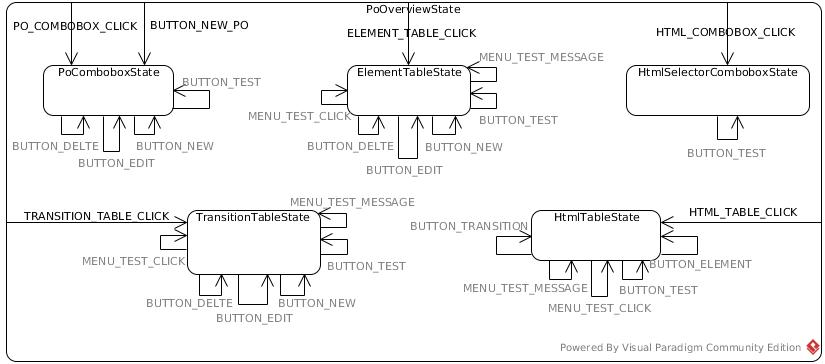
\includegraphics[scale=0.43]{img/StateMashine.jpg}\\
  \caption{Zustandsmodell des SeleniPoEditor}
  \label{fig:state_mashine}
\end{figure}

\begin{figure}[htb]
  \centering  
  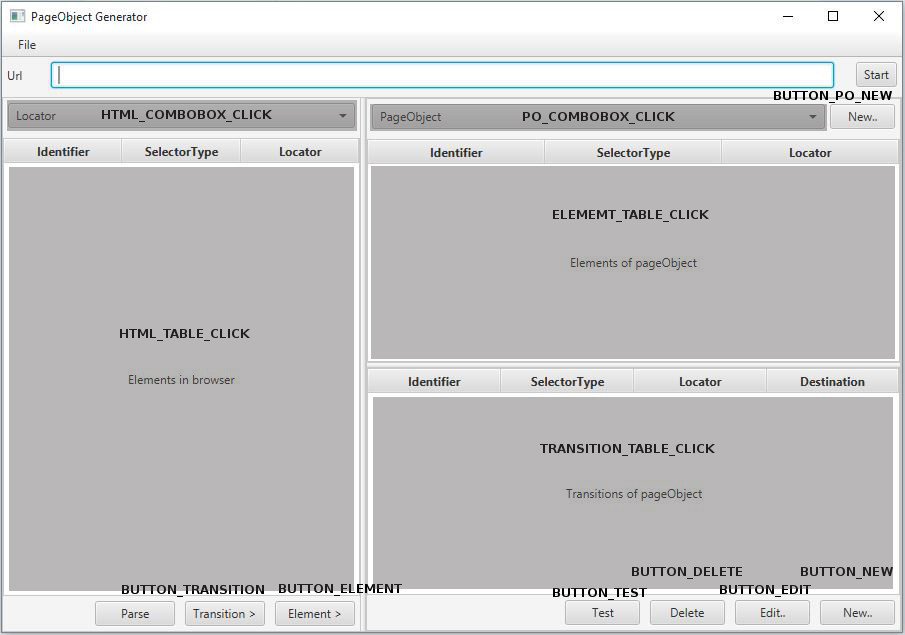
\includegraphics[scale=0.4]{img/poGeneratorEvents.jpg}\\
  \caption{Zuordnung der in Abbildung \ref{fig:state_mashine} verwendeten Namen }
  \label{fig:state_mashine_zuordnung}
\end{figure}

\newpage
\section{Vollständiges technisches Modell}
\label{anhang:vollständiges_technisches_modell}

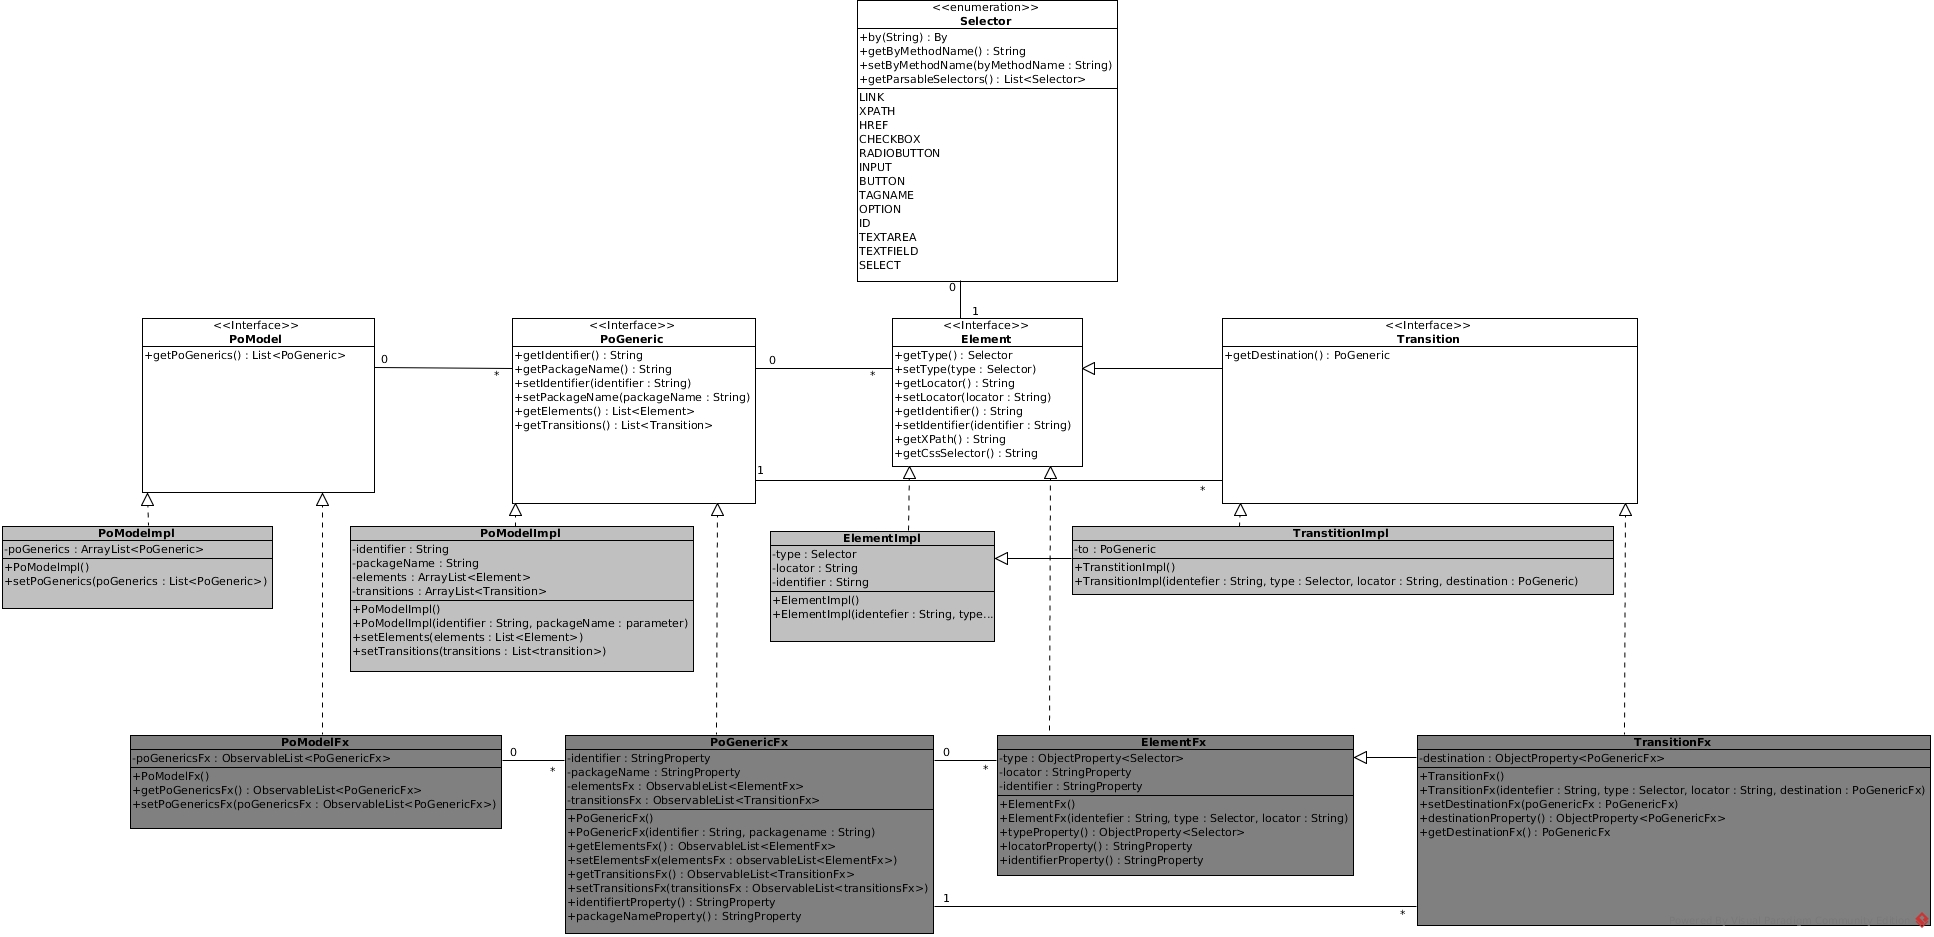
\includegraphics[angle=90,height=0.95\textheight]{img/ComplexModel.jpg}



\newpage

\section{Beispiel für ein Velocity Template}
\label{anhang:beispiel_velocity_template}
\begin{lstlisting}[caption={poGenerated.vm},label={lst:template_pogenerated}]
#set( $BASE_PACKAGE = $basePackagePath )
#set( $GENERATED_PACKAGE = "$BASE_PACKAGE#if ( $poGeneric.getPackageName() && $poGeneric.getPackageName().trim().size() != 0 ).$poGeneric.getPackageName()#end" )
#set( $EDIT_PACKAGE = "$BASE_PACKAGE" )
#set( $CLASS_NAME = "$poGeneric.getIdentifier()Generated" )

package $GENERATED_PACKAGE;

import ${BASE_PACKAGE}.BasePo;
import ${BASE_PACKAGE}.Control;
import ${BASE_PACKAGE}.PageObject;
#foreach( $destPo in $destionationPos )
import $EDIT_PACKAGE#if ( $destPo.getPackageName() && $destPo.getPackageName().trim().size() != 0 ).$destPo.getPackageName()#end.$destPo.getIdentifier();
#end

public class $CLASS_NAME extends BasePo {

#foreach( $element in $poGeneric.getElements() )
	public final Control $element.getIdentifier() = control(by.$element.getType().getByMethodName()("$element.getLocator()"));
#end
#foreach( $transition in $poGeneric.getTransitions() )
	public final Control $transition.getIdentifier() = control(by.$transition.getType().getByMethodName()("$transition.getLocator()"));
#end
	public $CLASS_NAME(PageObject po) {
		super(po);
	}
#foreach( $transition in $poGeneric.getTransitions() )
	
	public $transition.getDestination().getIdentifier() click${display.capitalize($transition.getIdentifier())}() {
		${transition.getIdentifier()}.click();
		return new $transition.getDestination().getIdentifier()(this);
	}
#end  
#foreach( $element in $poGeneric.getElements() )
	/**
	 * Get the Control for the Element $transition.getIdentifier().
	 * @return $transition.getIdentifier() - Element
	 */
	public Control get${display.capitalize($element.getIdentifier())}() {
		return $element.getIdentifier();
	}	
#end
#foreach( $transition in $poGeneric.getTransitions() )
	/**
	 * Get the Control for the Transition $transition.getIdentifier().
	 * @return $transition.getIdentifier() - Transition
	 */
	public Control get${display.capitalize($transition.getIdentifier())}() {
		return $transition.getIdentifier();
	}
	
#end
}

\end{lstlisting} 
\begin{lstlisting}[caption={poEditable.vm},label={lst:template_poeditable}]
#set( $BASE_PACKAGE = $basePackagePath )
#set( $EDIT_PACKAGE = "$BASE_PACKAGE#if ( $poGeneric.getPackageName() && $poGeneric.getPackageName().trim().size() != 0 ).$poGeneric.getPackageName()#end" )
#set( $GENERATED_PACKAGE = "$BASE_PACKAGE#if ( $poGeneric.getPackageName() && $poGeneric.getPackageName().trim().size() != 0 ).$poGeneric.getPackageName()#end" )
#set( $CLASS_NAME = "$poGeneric.getIdentifier()" )
#set( $CLASS_NAME_SUPER = "$poGeneric.getIdentifier()Generated" )

package $EDIT_PACKAGE;

import ${BASE_PACKAGE}.BasePo;
import ${BASE_PACKAGE}.Control;
import ${BASE_PACKAGE}.PageObject;
import $GENERATED_PACKAGE.$CLASS_NAME_SUPER;

public class $CLASS_NAME extends $CLASS_NAME_SUPER {

	public $CLASS_NAME(PageObject po) {
		super(po);
	}
}
\end{lstlisting} 